\documentclass[12pt]{article}

%--------------------------------------------------
% BASIC PACKAGES
%--------------------------------------------------
\usepackage[margin=1in]{geometry}      % Adjust page margins
\usepackage{amsmath,amssymb,amsfonts} % Math-related packages
\usepackage{graphicx}                 % For including images
\usepackage{booktabs}                 % For nicer tables
\usepackage{hyperref}                 % For hyperlinks in the PDF
\usepackage{enumitem}                 % For customizing lists
\usepackage{lipsum}                   % Example text (remove later)
\usepackage{tabularx}
\usepackage{float}
\usepackage{caption}
\usepackage{lscape} 
%--------------------------------------------------
% BASIC INFO
%--------------------------------------------------
\title{Macroeconomics Homework 1}
\author{Henry Su (b11303052)}
\date{\today}   % \today will auto-generate the current date

%--------------------------------------------------
% CUSTOM COMMANDS (OPTIONAL)
%--------------------------------------------------
% For example, a shortcut command for partial derivatives:
\newcommand{\pd}[2]{\frac{\partial #1}{\partial #2}}

% Or a shortcut for expectations in math mode:
\newcommand{\E}{\mathbb{E}}

%--------------------------------------------------
\begin{document}

%--------------------------------------------------
% TITLE
%--------------------------------------------------
\maketitle
\thispagestyle{empty}  % Remove page number from the title page if you like

%--------------------------------------------------
% INSTRUCTIONS
%--------------------------------------------------
% Provide instructions or an overview for your homework here.
% For example:
% "Please answer all questions clearly. Show all work."

\vspace{1cm} % Extra vertical space

%--------------------------------------------------
% PROBLEM 1
%--------------------------------------------------
\section*{Problem 1: Malthusian Model Simulation}
% State the problem you’re solving:
% For example:
% \lipsum[1] % placeholder text
\subsection*{(a): Creating Table for the first 15 period}
Note that one important assumption here is that all output $\mathrm{Y}$ is consumed by the labor force (i.e. $\mathrm{Y}_t$ = $\mathrm{C}_t$)
\begin{table}[H]
\centering
\caption{Malthusian Model Simulation Results}
\begin{tabular}{c|ccccccccc}
\toprule
period $t$ & $\mathrm{L}$ & $\mathrm{N}_t$ & $\mathrm{Y}_t$ & $\mathrm{C}_t$ & $\frac{\mathrm{C}_t}{\mathrm{N}_t}$ & Birth & Death & $\mathrm{N}_{t+1}$ & $\frac{\mathrm{L}}{\mathrm{N}_{t+1}}$\\
\midrule
0  & 100 & 50.00 & 10.10 & 10.10 & 0.2020 & 5.051 & 2.980 & 52.07 & 1.92 \\
1  & 100 & 52.07 & 10.31 & 10.31 & 0.1980 & 5.154 & 3.145 & 54.08 & 1.85 \\
2  & 100 & 54.08 & 10.51 & 10.51 & 0.1943 & 5.253 & 3.307 & 56.03 & 1.78 \\
3  & 100 & 56.03 & 10.69 & 10.69 & 0.1909 & 5.346 & 3.464 & 57.91 & 1.73 \\
4  & 100 & 57.91 & 10.87 & 10.87 & 0.1877 & 5.436 & 3.617 & 59.73 & 1.67 \\
5  & 100 & 59.73 & 11.04 & 11.04 & 0.1848 & 5.520 & 3.765 & 61.48 & 1.63 \\
6  & 100 & 61.48 & 11.20 & 11.20 & 0.1822 & 5.601 & 3.908 & 63.18 & 1.58 \\
7  & 100 & 63.18 & 11.35 & 11.35 & 0.1797 & 5.677 & 4.047 & 64.81 & 1.54 \\
8  & 100 & 64.81 & 11.50 & 11.50 & 0.1775 & 5.750 & 4.181 & 66.38 & 1.51 \\
9  & 100 & 66.38 & 11.64 & 11.64 & 0.1753 & 5.819 & 4.310 & 67.89 & 1.47 \\
10 & 100 & 67.89 & 11.77 & 11.77 & 0.1734 & 5.885 & 4.434 & 69.34 & 1.44 \\
11 & 100 & 69.34 & 11.90 & 11.90 & 0.1716 & 5.948 & 4.555 & 70.73 & 1.41 \\
12 & 100 & 70.73 & 12.01 & 12.01 & 0.1699 & 6.007 & 4.670 & 72.07 & 1.39 \\
13 & 100 & 72.07 & 12.13 & 12.13 & 0.1683 & 6.064 & 4.781 & 73.35 & 1.36 \\
14 & 100 & 73.35 & 12.23 & 12.23 & 0.1668 & 6.117 & 4.888 & 74.58 & 1.34 \\
15 & 100 & 74.58 & 12.34 & 12.34 & 0.1654 & 6.168 & 4.990 & 75.76 & 1.32 \\
\bottomrule
\end{tabular}
\end{table}
\subsection*{(b) Phase Diagram for Population ($N_t$ vs.\ $N_{t+1}$)}
\begin{figure}[H]
    \centering
    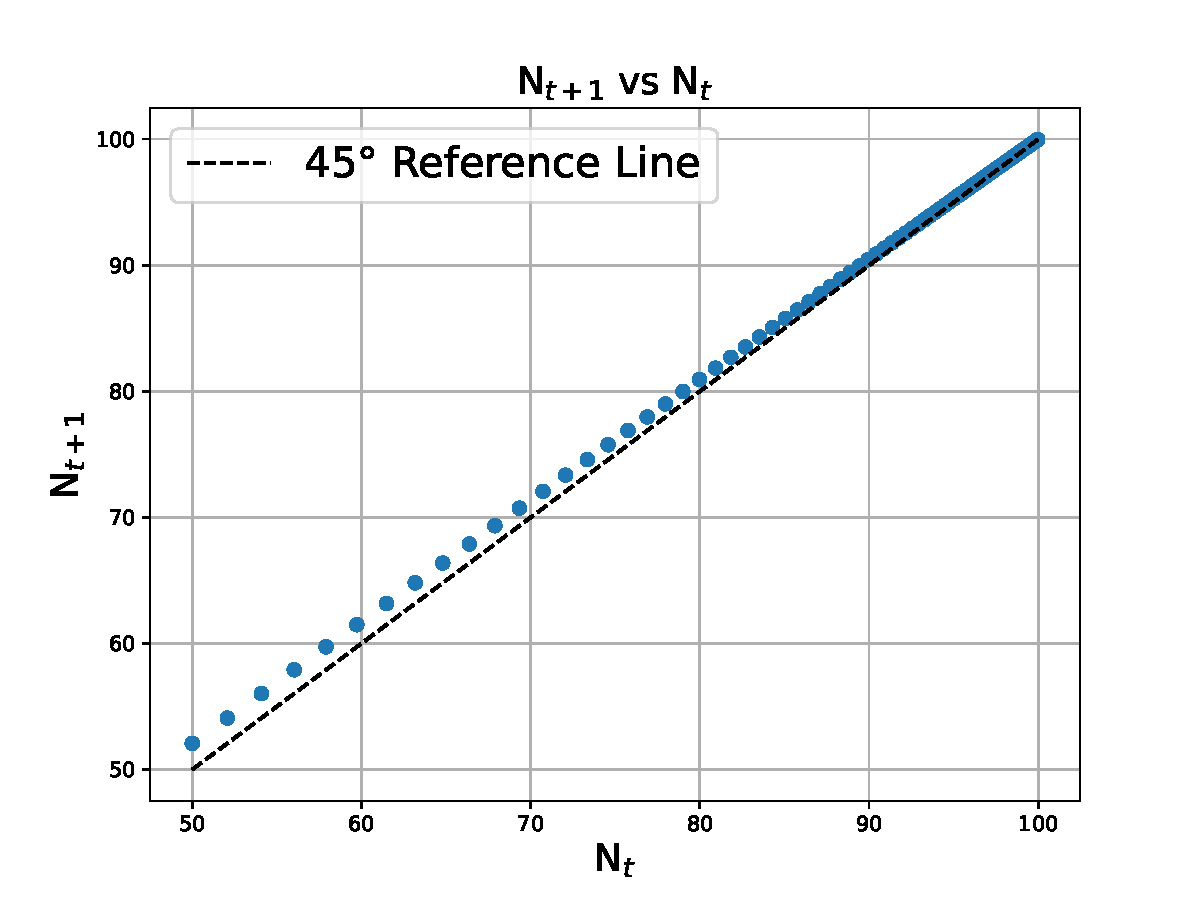
\includegraphics[width=0.7\textwidth]{1(b).pdf}
    \caption{Phase diagram plotting $N_{t+1}$ against $N_{t}$ with a 45$^\circ$ reference line,
    illustrating how the population evolves over time under the Malthusian model.
    Where the curve intersects the 45$^\circ$ line indicates a steady-state population.}
    \label{fig:nt_vs_ntplus1}
\end{figure}

\subsection*{(c) Time Paths of $N_t$ and $\frac{C_t}{N_t}$}
\begin{figure}[H]
    \centering
    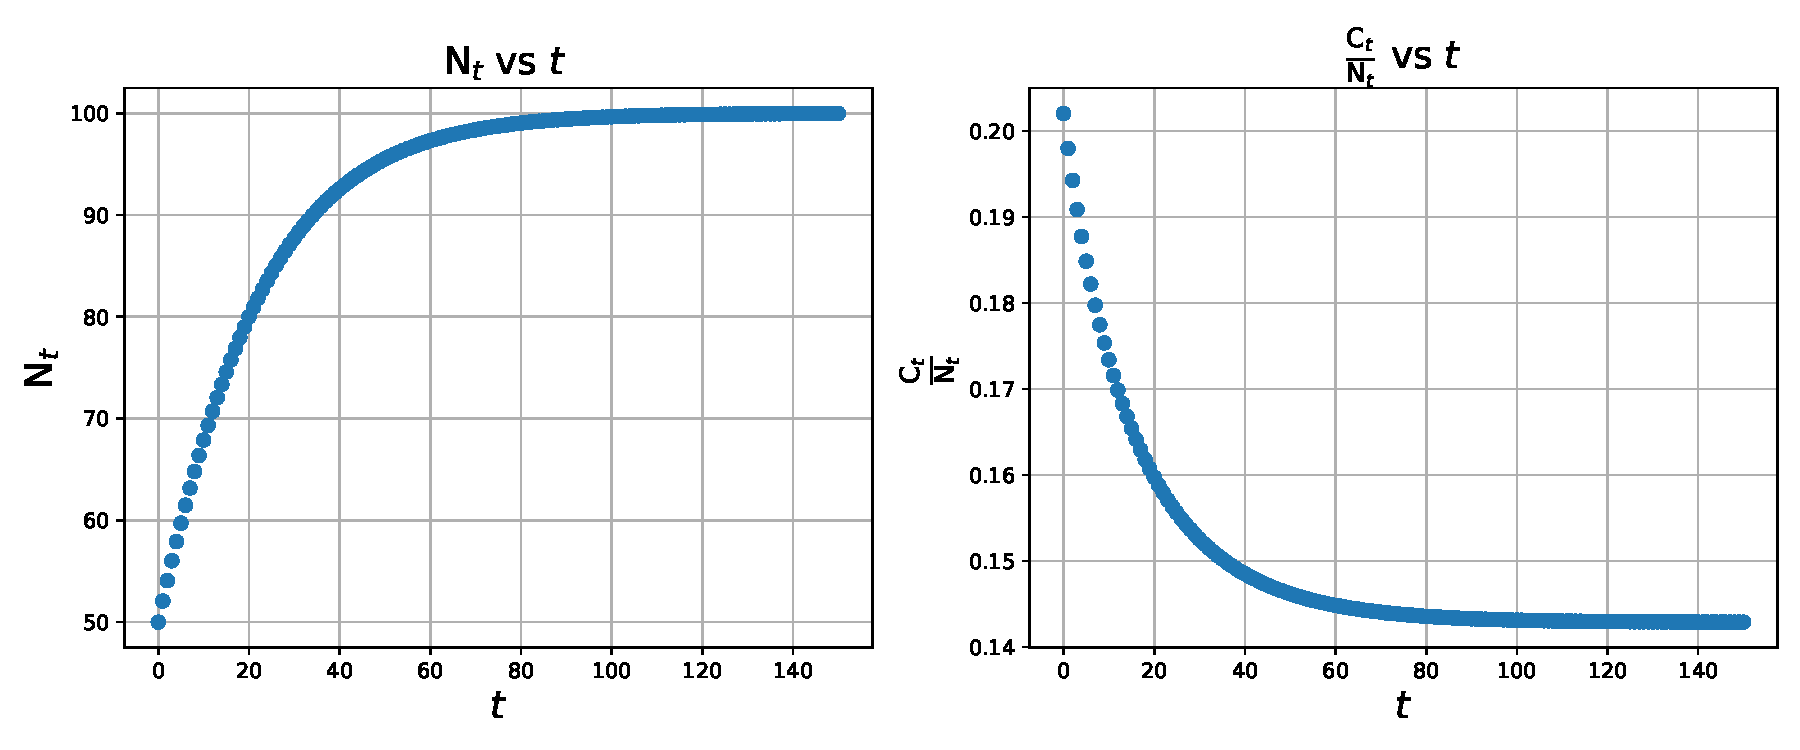
\includegraphics[width=1\textwidth]{1(c).pdf}
    \caption{Left panel: The evolution of population $N_t$ over time. 
    Right panel: Consumption per worker $\bigl(\tfrac{C_t}{N_t}\bigr)$ over time. 
    Both demonstrate how population growth and per‐worker consumption adjust in the Malthusian setting.}
    \label{fig:1(c)}
\end{figure}

\subsection*{(d) Effect of a Permanent TFP Shock ($z \to z'=5$ at $t=80$)}
\begin{figure}[H]
    \centering
    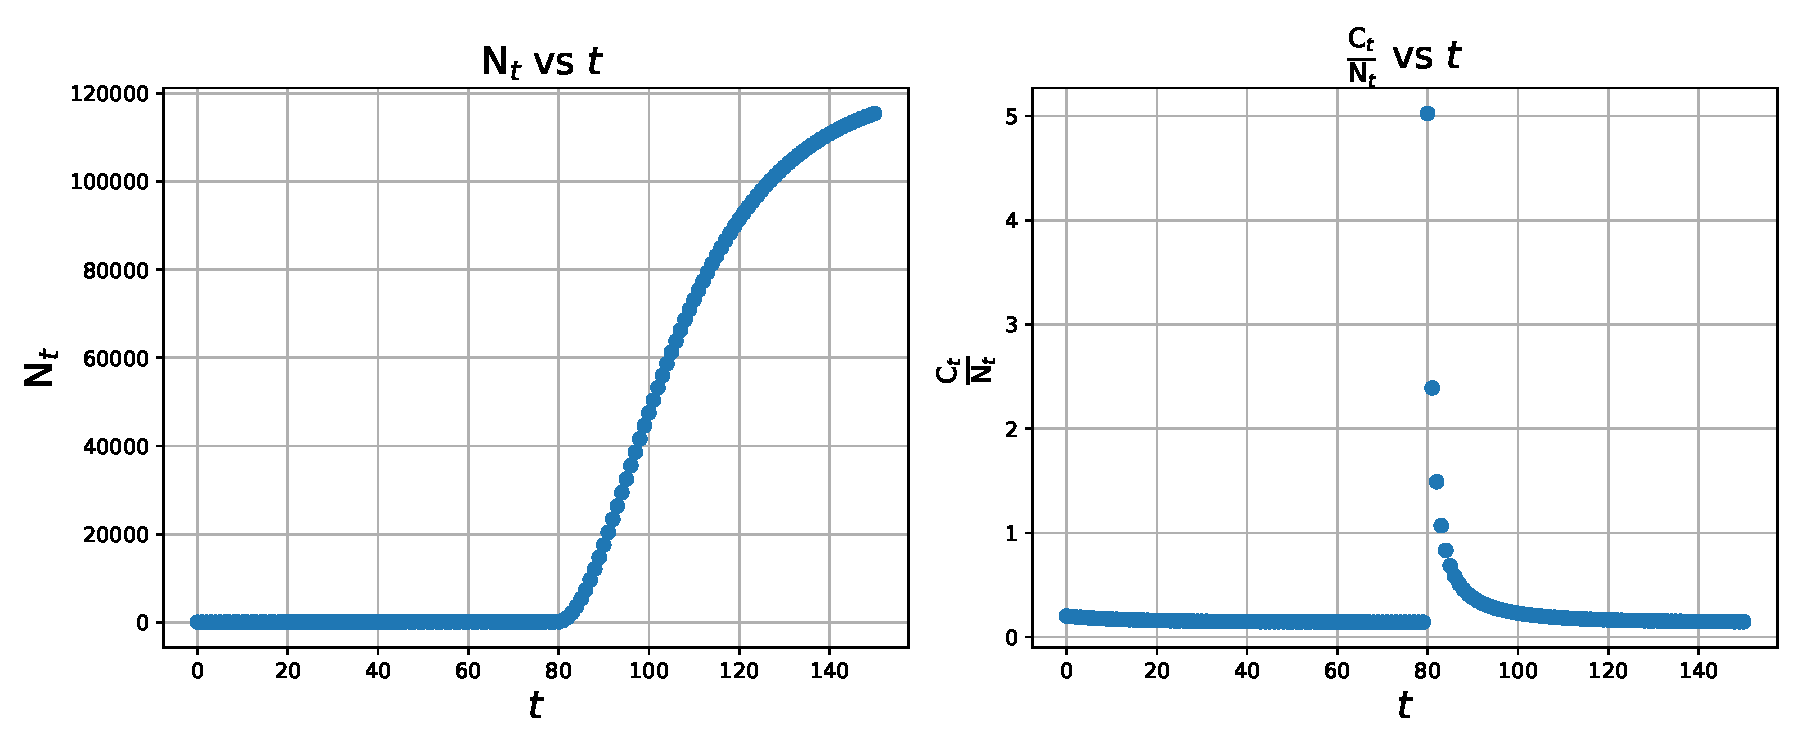
\includegraphics[width=1\textwidth]{1(d).pdf}
    \caption{After $t=80$, total factor productivity ($z$) permanently increases to 5. 
    The left panel shows how population $N_t$ grows more rapidly over time 
    under higher productivity, while the right panel depicts the resulting path 
    of consumption per worker $\tfrac{C_t}{N_t}$. 
    The new shock changes the long-run equilibrium in line with 
    Malthusian dynamics (more resources trigger faster population growth).}
    \label{fig:1(d)}
\end{figure}


%--------------------------------------------------
% PROBLEM 2
%--------------------------------------------------
\section*{Problem 2: Solow Model Simulation}
\subsection*{(a): Table for the first 15 period}
\begin{table}[H]
    \centering
    \caption{Solow Model Simulation Results}
    \space
    \resizebox{\textwidth}{!}{%

    \begin{tabular}{c|ccccccccccc}
    \hline
    period $t$ & $\mathrm{K}_t$ & $\mathrm{N}_t$ & $\frac{\mathrm{K}_t}{\mathrm{N}_t} = k_t$ & $\mathrm{Y}_t$ & $\mathrm{C}_t$ & $\mathrm{S}_t$& $\frac{\mathrm{C}_t}{\mathrm{N}_t} = c_t$ & $\mathrm{K}_{t+1}$& $\mathrm{N}_{t+1}$& $\mathrm{N}_{t+1}$ & $\frac{\mathrm{K}_{t+1}}{\mathrm{N}_{t+1}}$\\
    \hline

    0  & 1000.00  & 100.00  & 10.00  & 2529.82  & 1897.37  & 632.46  & 18.97  & 1332.46  & 120.00  & 120.00  & 11.10 \\
    1  & 1332.46  & 120.00  & 11.10  & 3198.95  & 2399.21  & 799.74  & 20.00  & 1732.46  & 144.00  & 144.00  & 12.03 \\
    2  & 1732.46  & 144.00  & 12.03  & 3995.79  & 2996.84  & 998.95  & 20.80  & 2211.67  & 172.80  & 172.80  & 12.80 \\
    3  & 2211.67  & 172.80  & 12.80  & 4945.63  & 3709.22  & 1236.41 & 21.45  & 2784.57  & 207.36  & 207.36  & 13.43 \\
    4  & 2784.57  & 207.36  & 13.43  & 6079.00  & 4559.25  & 1519.75 & 21.99  & 3468.95  & 248.83  & 248.83  & 13.95 \\
    5  & 3468.95  & 248.83  & 13.95  & 7432.62  & 5574.46  & 1858.16 & 22.40  & 4286.42  & 298.60  & 298.60  & 14.36 \\
    6  & 4286.42  & 298.60  & 14.36  & 9050.68  & 6788.01  & 2262.67 & 22.76  & 5263.16  & 358.32  & 358.32  & 14.69 \\
    7  & 5263.16  & 358.32  & 14.69  & 10986.21 & 8239.66  & 2746.55 & 23.00  & 6430.77  & 429.98  & 429.98  & 14.96 \\
    8  & 6430.77  & 429.98  & 14.96  & 13302.90 & 9977.17  & 3325.73 & 23.21  & 7827.26  & 515.98  & 515.98  & 15.18 \\
    9  & 7827.26  & 515.98  & 15.18  & 16077.20 & 12057.90 & 4019.30 & 23.38  & 9498.38  & 619.17  & 619.17  & 15.34 \\
    10 & 9498.38  & 619.17  & 15.34  & 19400.86 & 14550.64 & 4850.22 & 23.51  & 11499.09 & 743.01  & 743.01  & 15.48 \\
    11 & 11499.09 & 743.01  & 15.48  & 23383.98 & 17537.98 & 5846.00 & 23.61  & 13895.36 & 891.61  & 891.61  & 15.58 \\
    12 & 13895.36 & 891.61  & 15.58  & 28158.68 & 21119.01 & 7039.67 & 23.69  & 16766.42 & 1069.93 & 1069.93 & 15.67 \\
    13 & 16766.42 & 1069.93 & 15.67  & 33883.50 & 25412.63 & 8470.87 & 23.74  & 20207.37 & 1283.92 & 1283.92 & 15.74 \\
    14 & 20207.37 & 1283.92 & 15.74  & 40748.68 & 30561.51 & 10187.17& 23.79  & 24332.33 & 1540.70 & 1540.70 & 15.79 \\
    15 & 24332.33 & 1540.70 & 15.79  & 48982.52 & 36736.89 & 12245.63& 23.86  & 29278.26 & 1848.84 & 1848.84 & 15.83 \\
    \hline

    \end{tabular}}
    \end{table}

    \subsection*{(b) Phase Diagram ($k_t$ vs.\ $k_{t+1}$)}
    \begin{figure}[H]
        \centering
        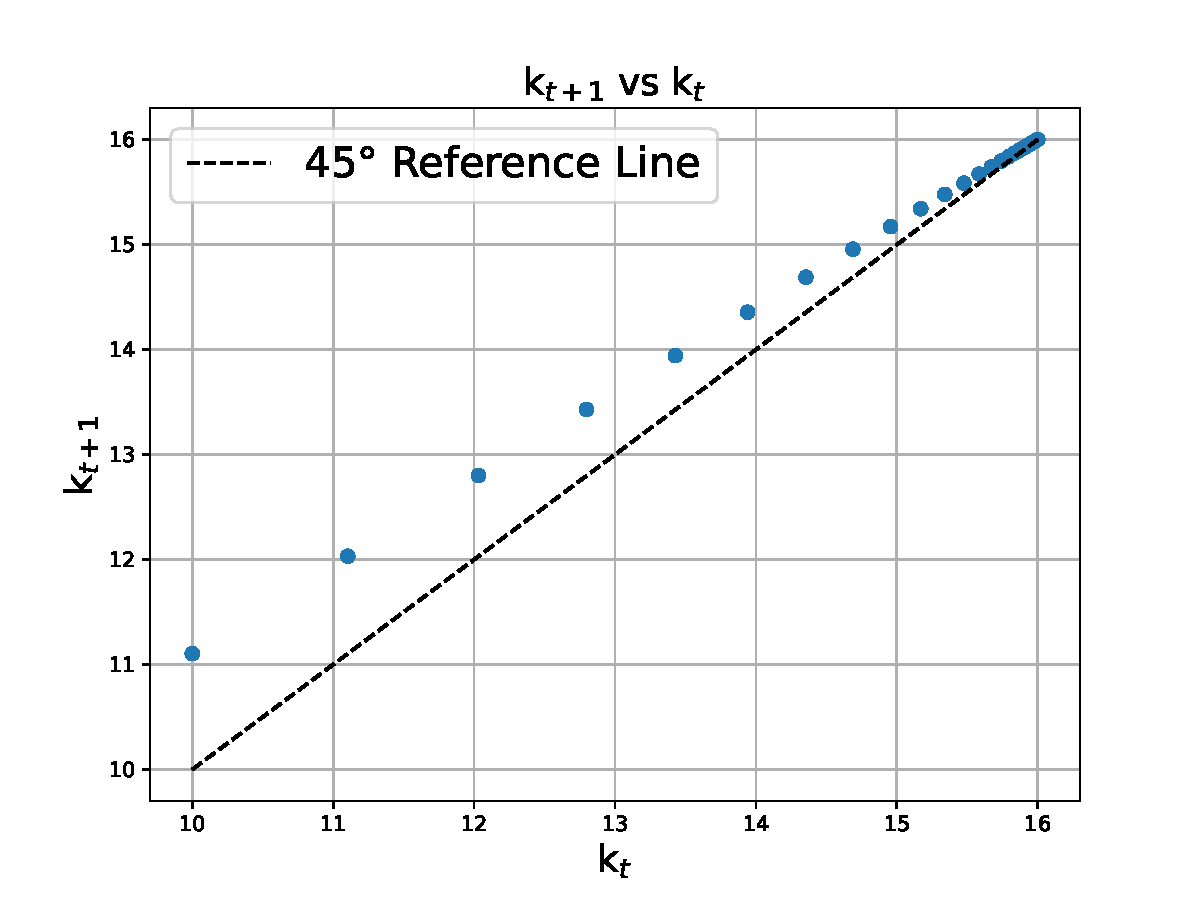
\includegraphics[width=0.7\textwidth]{2(b).pdf}
        \caption{Phase diagram plotting $k_{t+1}$ against $k_{t}$ with a 45$^{\circ}$ reference line, 
        illustrating how the economy converges to a steady-state capital per worker.}
        \label{fig:2(b)}
    \end{figure}
    
    \subsection*{(c) Time Paths of $k_t$ and $c_t$}
    \begin{figure}[H]
        \centering
        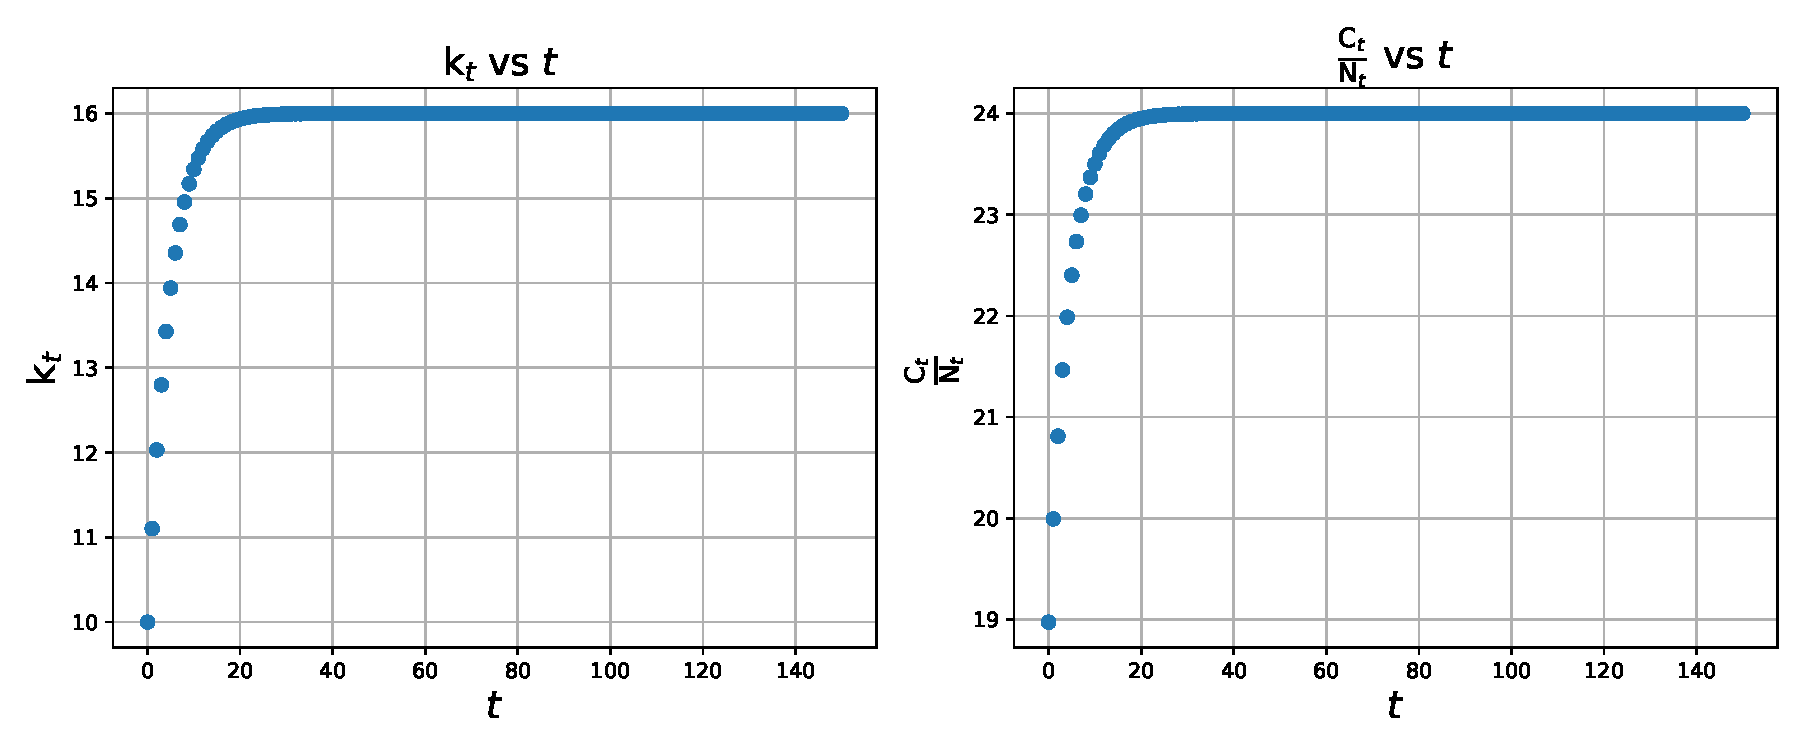
\includegraphics[width = 1\textwidth]{2(c).pdf}
        \caption{The left panel shows the evolution of $k_t$ (capital per worker) over time, 
        while the right panel shows the evolution of $c_t$ (consumption per worker) over time. 
        Both series converge to their respective steady-state values.}
        \label{fig:2(c)}
    \end{figure}
    
    \subsection*{(d) Effect of a Permanent TFP Shock ($z \to z'=5$ at $t=80$)}
    \begin{figure}[H]
        \centering
        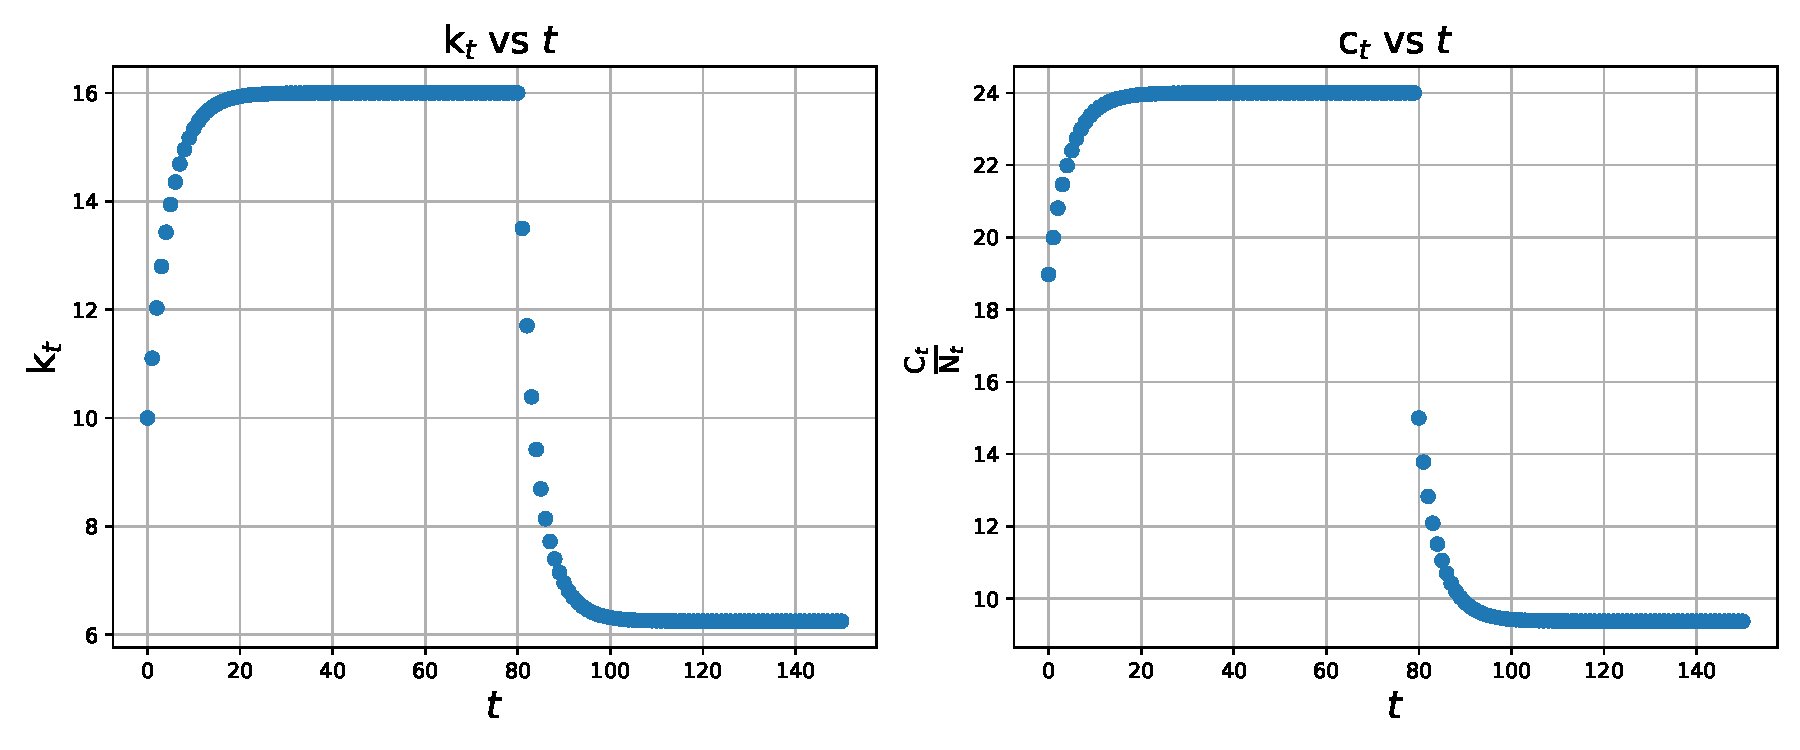
\includegraphics[width= 1\textwidth]{2(d).pdf}
        \caption{Impact of a permanent increase in TFP at $t=80$. 
        The figure re-plots $k_t$ and $c_t$ to show how the economy transitions to a new, 
        lower steady state.}
        \label{fig:2(d)}
    \end{figure}
    
    \subsection*{(e) Effect of a Permanent Increase in Savings Rate ($s \to s'=0.5$ at $t=80$)}
    \begin{figure}[H]
        \centering
        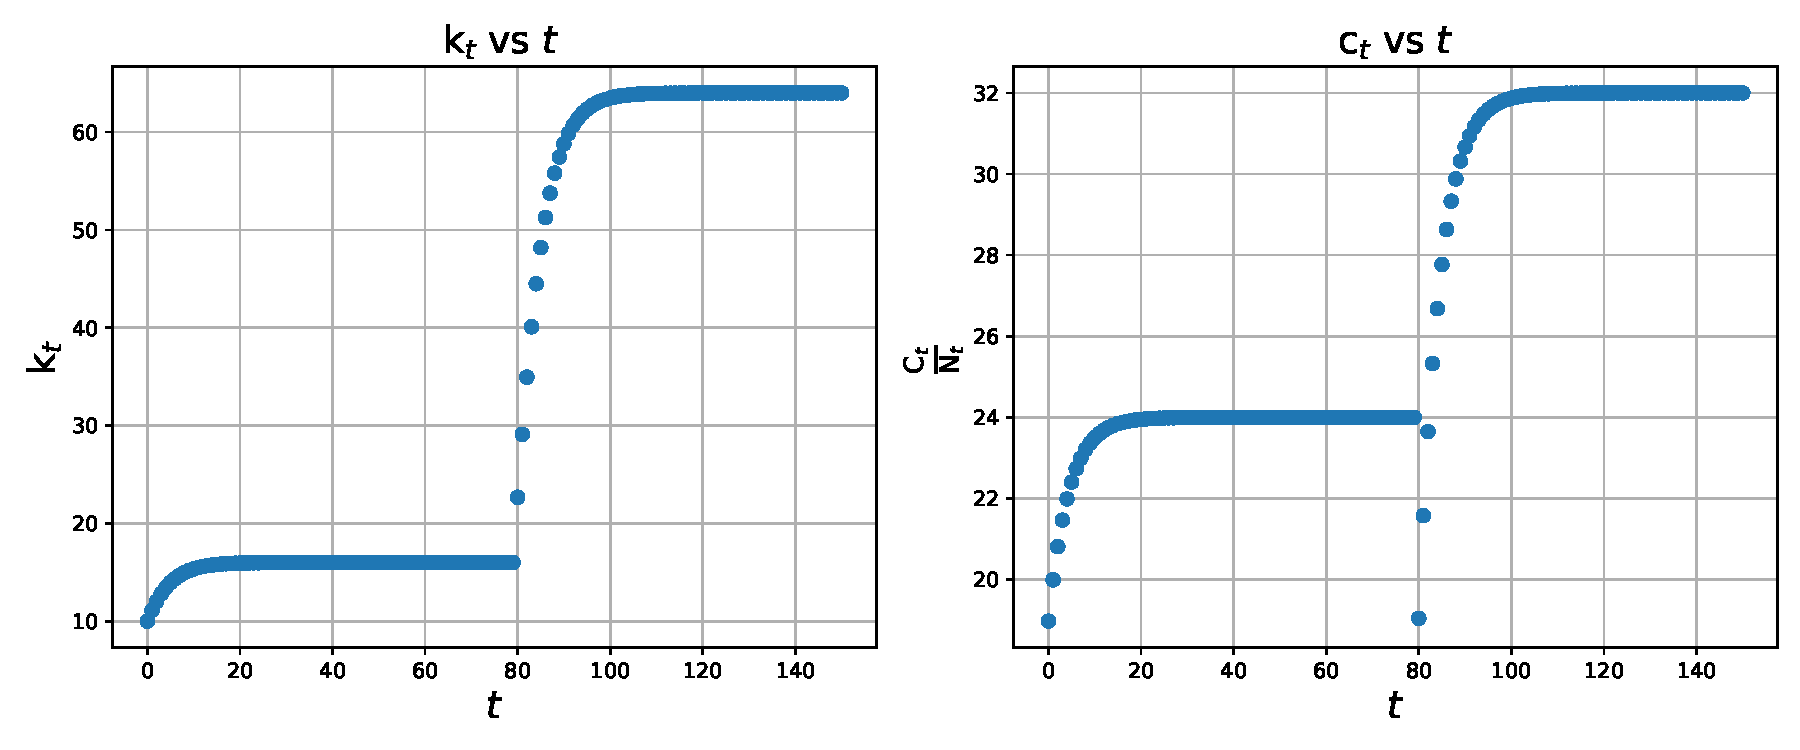
\includegraphics[width= 1\textwidth]{2(e).pdf}
        \caption{Illustration of a sudden increase in the savings rate $s$ from 0.25 to 0.5 at $t=80$.
        As savings rises, the capital stock $k_t$ grows faster, causing $c_t$ also to increase.
}
        \label{fig:2(e)}
    \end{figure}
% Example text:
% \lipsum[3]

%--------------------------------------------------
% Problem 3
%-------------------------------------------------

\section*{Problem 3: Hybrid Model}
\subsection*{(a): Table for the first 15 period}
\begin{table}[H]
    \centering
    \caption{Hybird Model Simulation Results}
    \space
    \resizebox{\textwidth}{!}{%

    \begin{tabular}{c|cccccccccccc}
    \hline
    period $t$ & $\mathrm{K}_t$ & $\mathrm{N}_t$ & $\frac{\mathrm{K}_t}{\mathrm{N}_t} = k_t$ & $\mathrm{Y}_t$ & $\mathrm{C}_t$ & $\mathrm{S}_t$& $\frac{\mathrm{C}_t}{\mathrm{N}_t} = c_t$ & $\frac{\mathrm{S}_t}{\mathrm{N}_{t}}$ & Net Population growth & $\mathrm{K}_{t+1}$& $\mathrm{N}_{t+1}$ & $\frac{\mathrm{K}_{t+1}}{\mathrm{N}_{t+1}}$\\
    \hline

    0  & 1000.00   & 100.00   & 10.00      & 2529.82   & 1897.37   & 632.46    & 18.97   & 6.32   & 0.00      & 1332.46   & 1038.68   & 1.28     \\
    1  & 1332.46   & 1038.68  & 1.28       & 9411.48   & 7058.61   & 2352.87   & 6.79    & 2.27   & 938.68    & 3285.59   & 4464.12   & 0.74     \\
    2  & 3285.59   & 4464.12  & 0.74       & 30638.29  & 22978.72  & 7659.57   & 5.15    & 1.72   & 4364.12   & 9959.48   & 15507.07  & 0.64     \\
    3  & 9959.48   & 15507.07 & 0.64       & 99419.88  & 74564.91  & 24854.97  & 4.81    & 1.60   & 15407.07  & 31826.61  & 51238.82  & 0.62     \\
    4  & 31826.61  & 51238.82 & 0.62       & 323061.14 & 242295.86 & 80765.29  & 4.73    & 1.58   & 51138.82  & 103043.91 & 167262.86 & 0.62     \\
    5  & 103043.91 & 167262.86& 0.62       & 1050269.91& 787702.43 & 262567.48 & 4.71    & 1.57   & 167162.86 & 334698.22 & 544387.79 & 0.61     \\
    6  & 334698.22 & 544387.79& 0.61       & 3414844.04& 2561133.03& 853711.01 & 4.71    & 1.57   & 544287.79 & 1087999.76& 1770515.53& 0.61     \\
    7  & 1087999.76& 1770515.53&0.61       & 1.110e+07 & 8.328e+06 & 2.776e+06 & 4.70    & 1.57   & 1770415.53& 3537438.79& 5757222.40& 0.61     \\
    8  & 3537438.79& 5757222.40&0.61       & 3.610e+07 & 2.707e+07 & 9.026e+06 & 4.71    & 1.57   & 5757122.40& 1.150e+07 & 1.8720e+07& 0.61     \\
    9  & 1.150e+07 & 1.8720e+07&0.61       & 1.1739e+08& 8.8042e+07& 2.9347e+07& 4.70    & 1.57   & 1.8720e+07& 3.7399e+07& 6.0869e+07& 0.61     \\
    10 & 3.7399e+07& 6.0869e+07&0.61       & 3.8169e+08& 2.8627e+08& 9.5424e+07& 4.70    & 1.57   & 6.0869e+07& 1.2160e+08& 1.9792e+08& 0.61     \\
    11 & 1.2160e+08& 1.9792e+08&0.61       & 1.2411e+09& 9.3082e+08& 3.1027e+08& 4.70    & 1.57   & 1.9792e+08& 3.9539e+08& 6.4354e+08& 0.61     \\
    12 & 3.9539e+08& 6.4354e+08&0.61       & 4.0354e+09& 3.0266e+09& 1.0089e+09& 4.70    & 1.57   & 6.4354e+08& 1.2856e+09& 2.0925e+09& 0.61     \\
    13 & 1.2856e+09& 2.0925e+09&0.61       & 1.3121e+10& 9.8410e+09& 3.2803e+09& 4.70    & 1.57   & 2.0925e+09& 4.1803e+09& 6.8037e+09& 0.61     \\
    14 & 4.1803e+09& 6.8037e+09&0.61       & 4.2665e+10& 3.1998e+10& 1.0666e+10& 4.70    & 1.57   & 6.8036e+09& 1.3592e+10& 2.2123e+10& 0.61     \\
    15 & 1.3592e+10& 2.2123e+10&0.61       & 1.3873e+11& 1.0404e+11& 3.4681e+10& 4.70    & 1.57   & 2.2123e+10& 4.4196e+10& 7.1932e+10& 0.61     \\
    \hline

    \end{tabular}}
    \end{table}
    \subsection*{(b) Time Paths of $k_t$, $c_t$, and $N_t$}
    \begin{figure}[H]
        \centering
        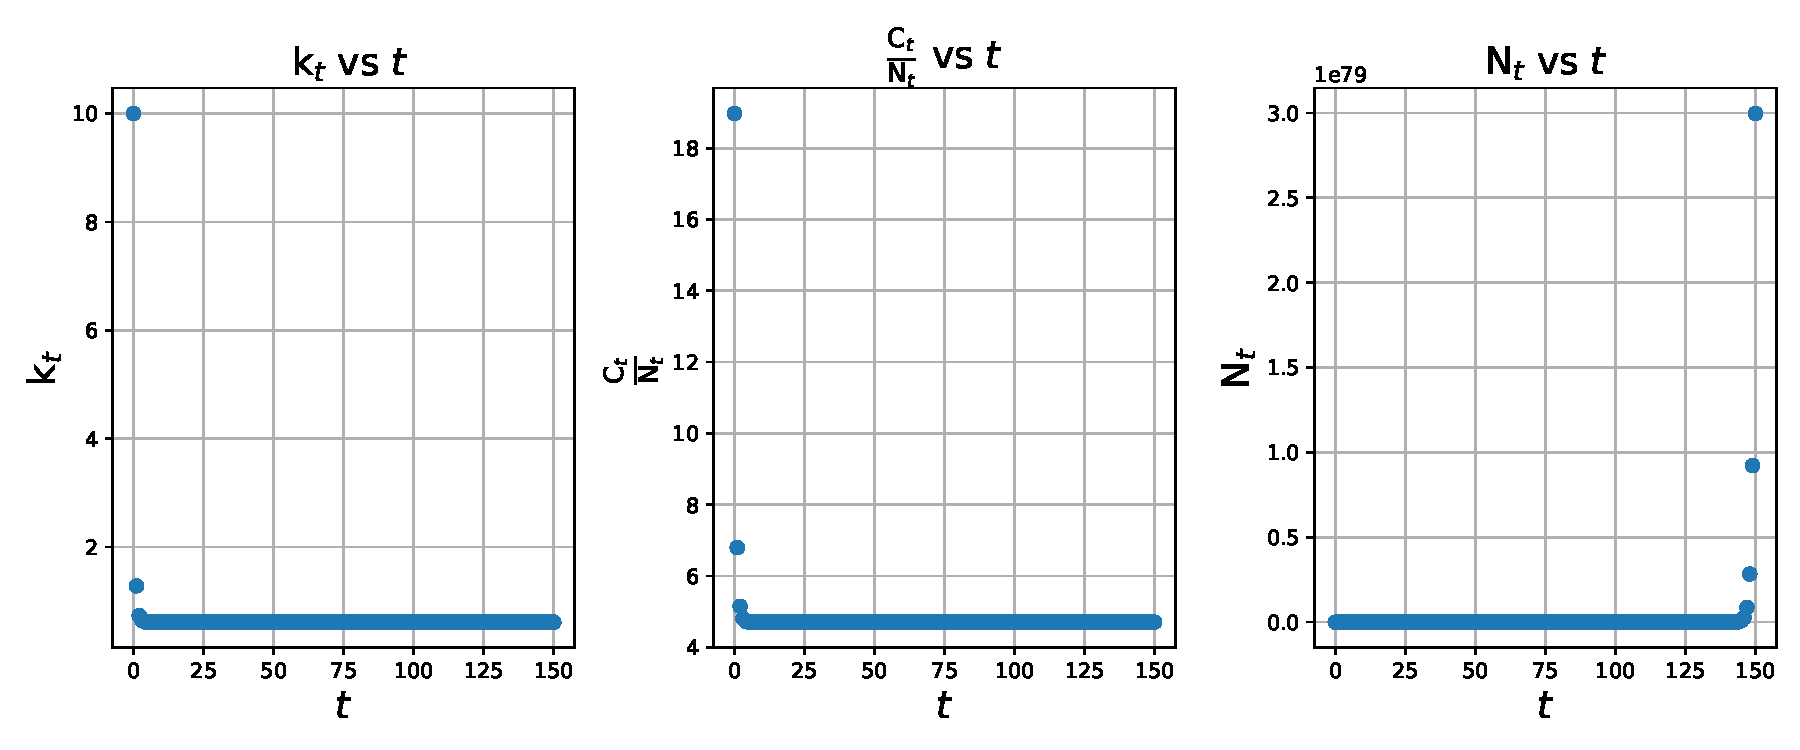
\includegraphics[width=1\textwidth]{3(b).pdf}
        \caption{In the hybrid model, population growth is endogenous. 
        Plots show how $k_t$, $c_t$, and $N_t$ evolve over time 
        and tend toward a particular growth path.}
        \label{fig:3(b)}
    \end{figure}
    
    \subsection*{(c) Effect of a Permanent TFP Shock ($z \to z'=5$ at $t=80$)}
    \begin{figure}[H]
        \centering
        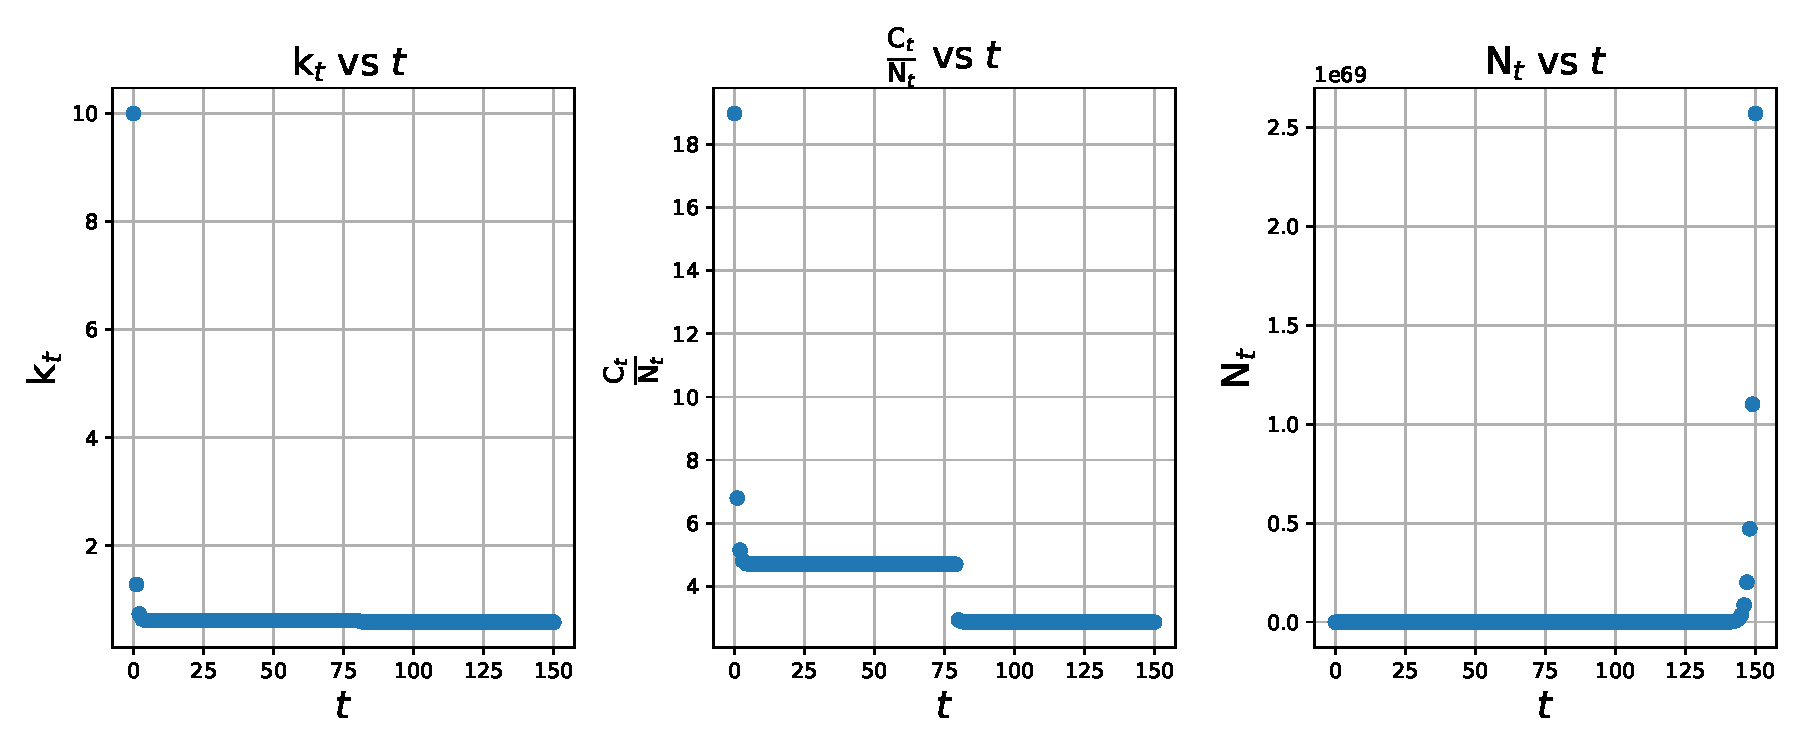
\includegraphics[width=1\textwidth]{3(c).pdf}
        \caption{Impact of a permanent increase in TFP at $t=80$ on $k_t$, $c_t$, and $N_t$ 
        in the hybrid model. Lower productivity decreases output, alters the saving/population 
        dynamics, and shifts the paths of all three variables.}
        \label{fig:3(c)}
    \end{figure}
    
    \subsection*{(d) Effect of a Permanent Increase in Savings Rate ($s \to s'=0.5$ at $t=80$)}
    \begin{figure}[H]
        \centering
        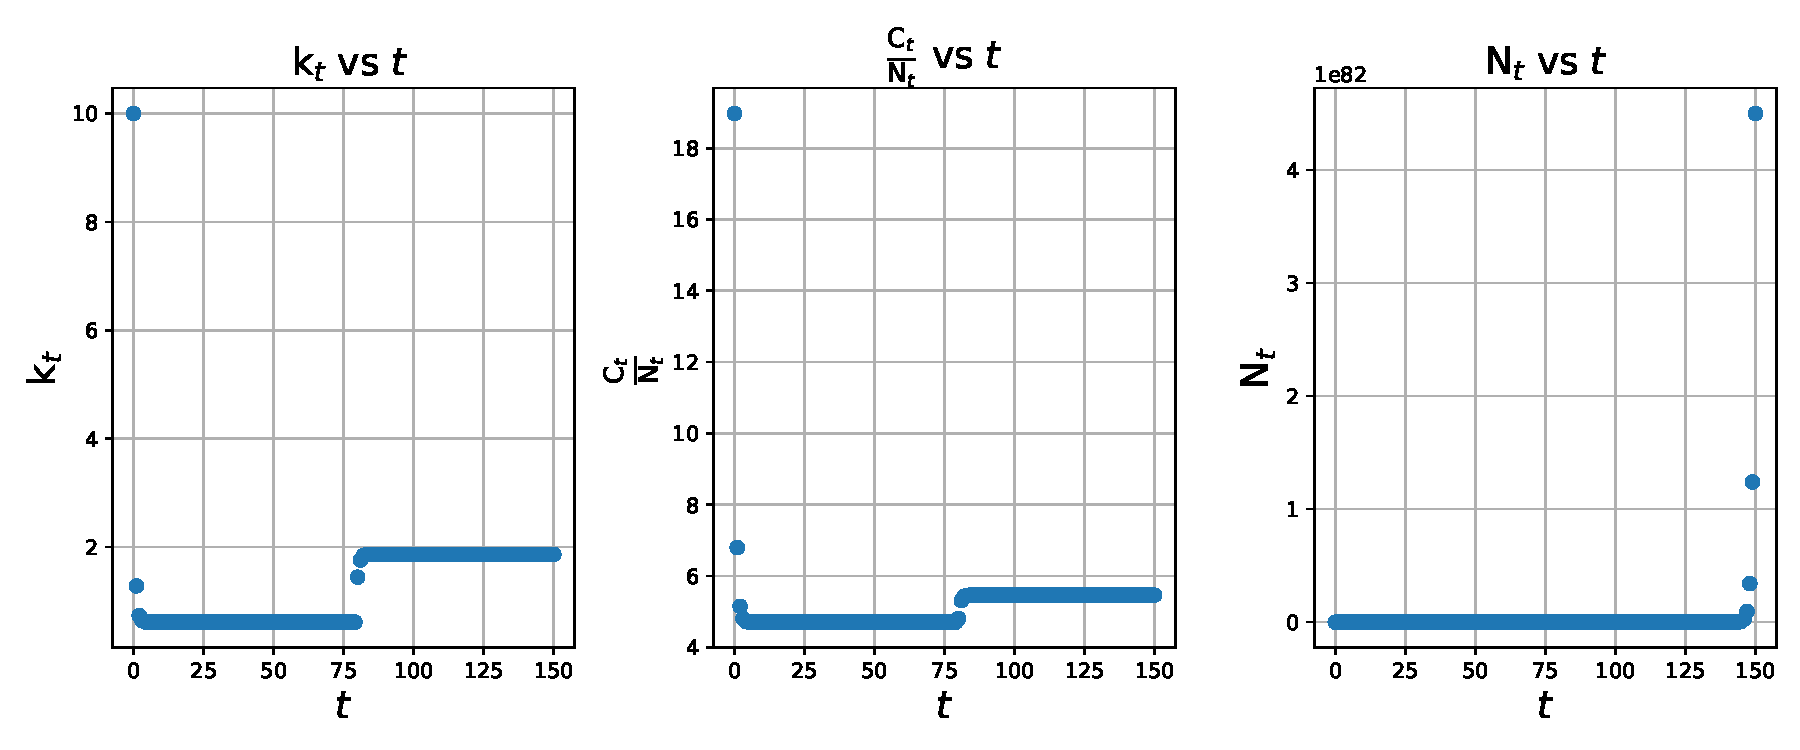
\includegraphics[width=1\textwidth]{3(d).pdf}
        \caption{The saving rate $s$ increases from 0.25 to 0.5 at $t=80$ in the hybrid model.
        More saving raises investment, causing $k_t$ to grow more quickly and eventually shift 
        upward, which also changes population growth and consumption dynamics over time.}
        \label{fig:3(d)}
    \end{figure}
\section*{Problem 4: Hand Calculation of TFP Solow Model}
\subsection*{(a): Law of motion of capital per effective worker}
Starting from the law of motion of captial:
\begin{equation}
    \mathrm{K}_{t+1} = (1-\delta)\mathrm{K}_t + s\mathrm{Y}_t
\end{equation}
Then, we divided by the effective worker which is,
\begin{equation}
    \mathrm{z}_{t+1}\mathrm{N}_{t+1}
\end{equation}
We have,
\begin{equation}
    \tilde{\mathrm{k}}_{t+1} = (1-\delta)\frac{\mathrm{K}_t}{\mathrm{z}_{t+1}\mathrm{N}_{t+1}} + s\frac{\mathrm{Y}_t}{\mathrm{z}_{t+1}\mathrm{N}_{t+1}}
    \label{equation:(3)}
\end{equation}
Looking at eq.\ref{equation:(3)}, we can simplify with the fact that production function is $\mathrm{Y}_t = \mathrm{K}_t^{\alpha}(\mathrm{z}_t\mathrm{N}_t^{1-\alpha})$. And $\frac{\mathrm{Y}_t}{\mathrm{z}_{t+1}\mathrm{N}_{t+1}} = \frac{\tilde{\mathrm{k}}_t^{\alpha}}{(1+g)(1+n)}$. Now, we have law of motion of capital per effective worker :
\begin{equation}
    \tilde{\mathrm{k}}_{t+1} = \frac{(1-\delta)\tilde{\mathrm{k}}_t + s\tilde{\mathrm{k}}_t^{\alpha}}{(1+g)(1+n)} \Rightarrow  \tilde{\mathrm{k}}_{t+1}(1+g)(1+n) = (1-\delta)\tilde{\mathrm{k}}_t + s\tilde{\mathrm{k}}_t^{\alpha}
    \label{equation:(4)}
\end{equation}
\subsection*{(b): Golden-rule saving rate to maximize $\tilde{\mathrm{c}}_t$}
Recall that the golden-rule saving rate suggest the saving rate that maximize steady-state consumption per effective worker. \\
Now we write the law of motion for consumption per effective worker for steady-state as follow,
\begin{equation}
    \tilde{\mathrm{k}}_{t+1}^{\star}(1+g)(1+n) = (1-\delta)\tilde{\mathrm{k}}_t^{\star} + s\tilde{\mathrm{k}}_t^{\star\alpha}
\end{equation}
Note that the steady-state for capital per effective worker is as follow:
\begin{equation}
    \tilde{\mathrm{k}}_{t+1}^{\star} = \tilde{\mathrm{k}}_{t}^{\star} = \tilde{\mathrm{k}}^{\star}
    \label{equation:(5)}
\end{equation}
So we can rewrite the equation as follow:
\begin{equation}
    \tilde{\mathrm{k}}^{\star}(1+g)(1+n) = (1-\delta)\tilde{\mathrm{k}}^{\star} + s\tilde{\mathrm{k}}^{\star\alpha} \Rightarrow (g+n+ng+\delta)\tilde{\mathrm{k}}^{\star} =  s\tilde{\mathrm{k}}^{\star\alpha} 
    \label{equation:(6)}
\end{equation}

\begin{equation}
    \tilde{\mathrm{c}}^{\star} = \tilde{\mathrm{y}}^{\star} - savings =  \tilde{\mathrm{y}}^{\star} - s\tilde{\mathrm{k}}_t^{\star\alpha} = \tilde{\mathrm{y}}^{\star} - (g+n+ng+\delta)\tilde{\mathrm{k}}^{\star} 
\end{equation}

And from maximized condition mentioned in class(equation 5, solow ppt page 23/36) the consumption is maximized when,
\begin{equation}
    \tilde{\mathrm{y}}^{\prime\star} = (g+n+ng+\delta)
\end{equation}
And because $\mathrm{y}_t^{\star} = \frac{\mathrm{Y}_t}{\mathrm{z}_{t}\mathrm{N}_{t}} = \tilde{\mathrm{k}}_t^{\alpha}$, we can rewrite the equation as follow:
\begin{equation}
    \tilde{\mathrm{y}}^{\prime\star} = \alpha\tilde{\mathrm{k}}^{\star(\alpha-1)} = g+n+ng+\delta
    \label{equation:(7)}
\end{equation} 
Then $\tilde{k}^{\star} = (\frac{\alpha}{n+g+ng+\delta})^{\frac{1}{1-\alpha}}$ and by eq.\ref{equation:(7)} we have,
\begin{equation*}
    s_{GR} = \alpha
\end{equation*}
\subsection*{(c): Growth rate of key variables in the steady state}
\subsubsection*{{(i): Growth rate of $\tilde{\mathrm{y}_t}$ and $\tilde{\mathrm{k}_t}$}}
In steady-state output per effective worker is constant becasue in steady-state captial per effective worker is constant(eq.\ref{equation:(6)}), so we have:
\begin{equation}
    \frac{\mathrm{Y}_{t+1}}{\mathrm{z}_{t+1}\mathrm{N}_{t+1}} = \frac{\mathrm{Y}_t}{\mathrm{z}_t\mathrm{N}_t} = \tilde{\mathrm{k}}^{\star\alpha} = constant
\end{equation}
So growth rate of $\tilde{\mathrm{y}_t}$ and $\tilde{\mathrm{k}_t}$ $= 0 $
\subsubsection*{{(ii): Growth rate of $\mathrm{y}_t$ and $\mathrm{k}_t$}}
Growth rate of $\mathrm{y}_t$ and $\mathrm{k}_t$ is define as follow(note that $\mathrm{k}_{t+1} = \mathrm{k}_{t} = constant $ in steady-state):
\begin{equation}
    \frac{\mathrm{y}_{t+1}}{\mathrm{y}_t} - 1 = \frac{\mathrm{z}_{t+1}\mathrm{k}_{t+1}^{\alpha}}{\mathrm{z}_t\mathrm{k}_t^{\alpha}} - 1  = 1 + g - 1 = g 
\end{equation}
\subsubsection*{{(ii): Growth rate of $\mathrm{K}_t$ and $\mathrm{Y}_t$}}
Growth rate of $\mathrm{Y}_t$ and $\mathrm{K}_t$ is define as follow:
\begin{equation}
    \frac{\mathrm{Y}_{t+1}}{\mathrm{Y}_t} - 1 = \frac{\mathrm{y}_{t+1}\mathrm{N}_{t+1}}{\mathrm{y}_t\mathrm{N}_t} - 1  = (1 + g)(1 + n) - 1 = n + g + ng 
\end{equation}
\subsection*{(d): Market clearing condition with government}
Recall before the assumption of a government present the market clearing conditions is:
\begin{equation}
    \mathrm{Y}_t = \mathrm{C}_t + \mathrm{I}_t
\end{equation}
Now with the present of a government, we have:
\begin{equation}
    \mathrm{Y}_t = \mathrm{C}_t + \mathrm{I}_t + \mathrm{G}_t
\end{equation}
Where $\mathrm{G}_t$ is the government spending. And we can rewrite the equation as follow:
\begin{equation}
    \mathrm{Y}_t = \mathrm{C}_t + \mathrm{I}_t + \mathrm{G}_t = \mathrm{C}_t + \mathrm{I}_t + \tau\mathrm{Y}_t
\end{equation}
\subsection*{(e): Law of motion of capital per effective worker with government}
The law of motion of capital per effective worker with government is similar to the one without government, but we need to minus the government spending in the term of investments. \\
So that's law of motion of captial is:
\begin{equation}
    \mathrm{K}_{t+1} = (1-\delta)\mathrm{K}_t + s(1 - \tau)\mathrm{Y}_t
\end{equation}
Then we divided by the effective worker which is,
\begin{equation}
    \mathrm{z}_{t+1}\mathrm{N}_{t+1}
\end{equation}
We have,
\begin{equation}
    \tilde{\mathrm{k}}_{t+1} = (1-\delta)\frac{\mathrm{K}_t}{\mathrm{z}_{t+1}\mathrm{N}_{t+1}} + s(1 - \tau)\frac{\mathrm{Y}_t}{\mathrm{z}_{t+1}\mathrm{N}_{t+1}}
    \label{equation:(19)}
\end{equation}
Can from the result we got in eq.\ref{equation:(4)}, we can rewrite the equation as follow:
\begin{equation}
    \tilde{\mathrm{k}}_{t+1} = \frac{(1-\delta)\tilde{\mathrm{k}}_t + s(1 - \tau)\tilde{\mathrm{k}}_t^{\alpha}}{(1+g)(1+n)} \Rightarrow  \tilde{\mathrm{k}}_{t+1}(1+g)(1+n) = (1-\delta)\tilde{\mathrm{k}}_t + s(1 - \tau)\tilde{\mathrm{k}}_t^{\alpha}
    \label{equation:(20)}
\end{equation}
Then we are done with the law of motion of capital per effective worker with government. \\

$\star$Note that if $ng$ is small, we can ignore the $ng$ term in all the equations above. \\
\subsection*{(f): Simulation of the model with government}
\subsubsection*{(i): Approxmate steady state}
we solve the approxmate steady state by using the following equation:
\begin{equation}
    \tilde{\mathrm{k}}^{\star} = \frac{s(1 - \tau)}{n+g+\delta}\tilde{\mathrm{k}}^{\star\alpha} \Rightarrow \tilde{\mathrm{k}}^{\star} = (\frac{s(1 - \tau)}{n+g+\delta})^{\frac{1}{1-\alpha}}
\end{equation}
With the value given. We can get:
\begin{equation}
    \tilde{k}_t^{\star}  \thickapprox 0.13
\end{equation}
\subsubsection*{(ii) Time Path of $\widetilde{k}_t$}
\begin{figure}[H]
    \centering
    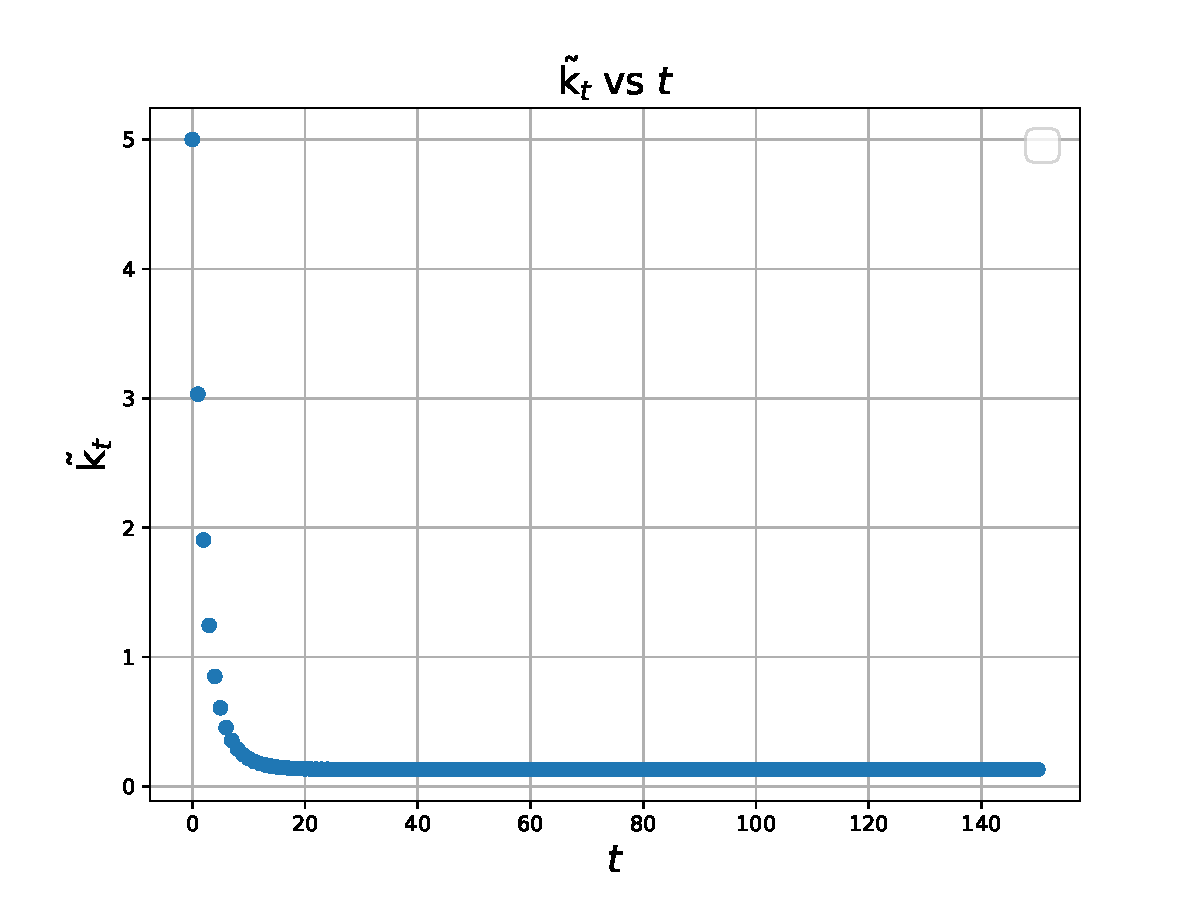
\includegraphics[width=0.7\textwidth]{4(f)(ii).pdf}
    \caption{The evolution of capital per effective worker, $\widetilde{k}_t$, over time. 
    As $t$ increases, $\widetilde{k}_t$ converges to a steady-state level determined 
    by the chosen parameters $(s, \alpha, \delta, n, g, \tau)$.}
    \label{fig:4(ii)}
\end{figure}

\subsubsection*{(iii) Time Path of $\widetilde{c}_t$}
\begin{figure}[H]
    \centering
    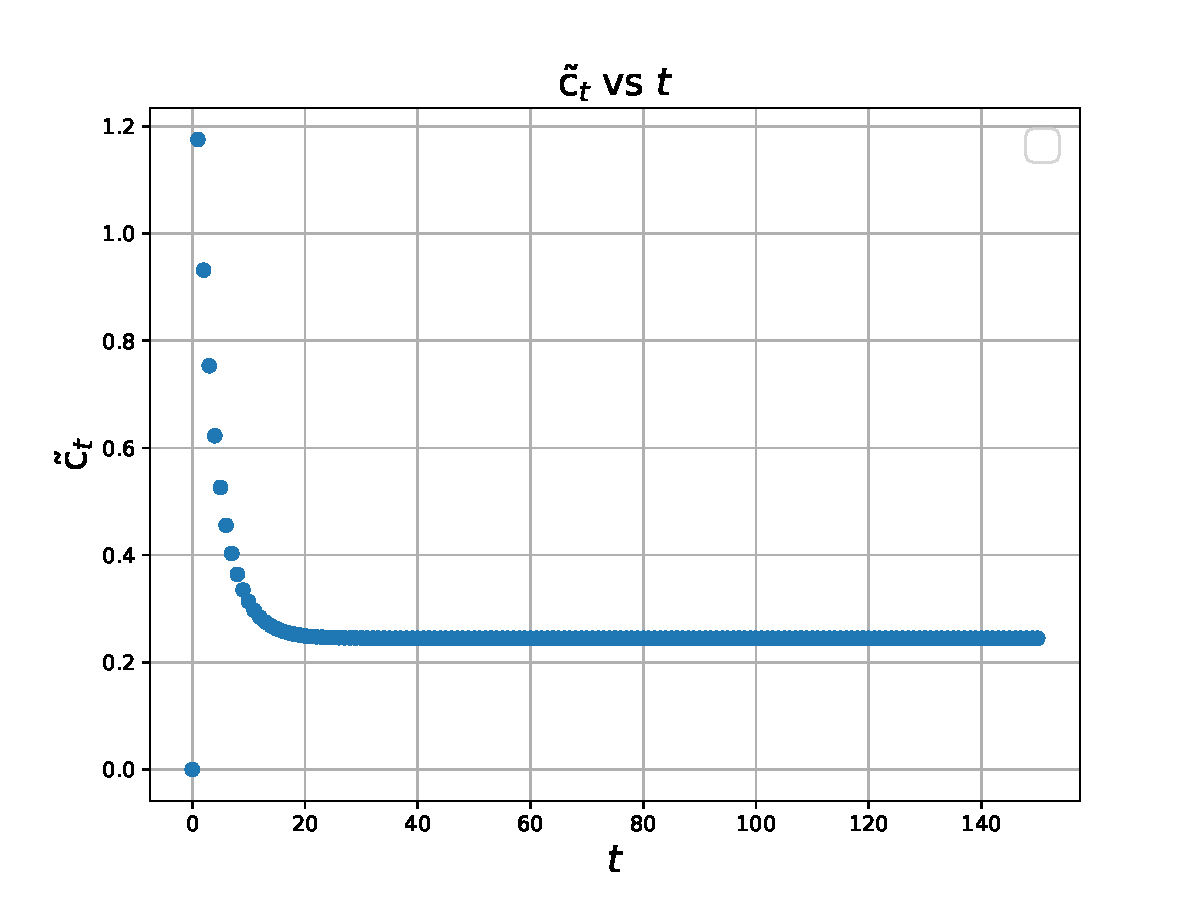
\includegraphics[width=0.7\textwidth]{4(f)(iii).pdf}
    \caption{The evolution of consumption per effective worker, $\widetilde{c}_t$, over time. 
    As the economy accumulates capital and productivity grows, $\widetilde{c}_t$ converges 
    to its long-run path in tandem with $\widetilde{k}_t$.}
    \label{fig:4(iii)}
\end{figure}

\subsection*{(g) Effect of Varying $\tau$}
\begin{figure}[H]
    \centering
    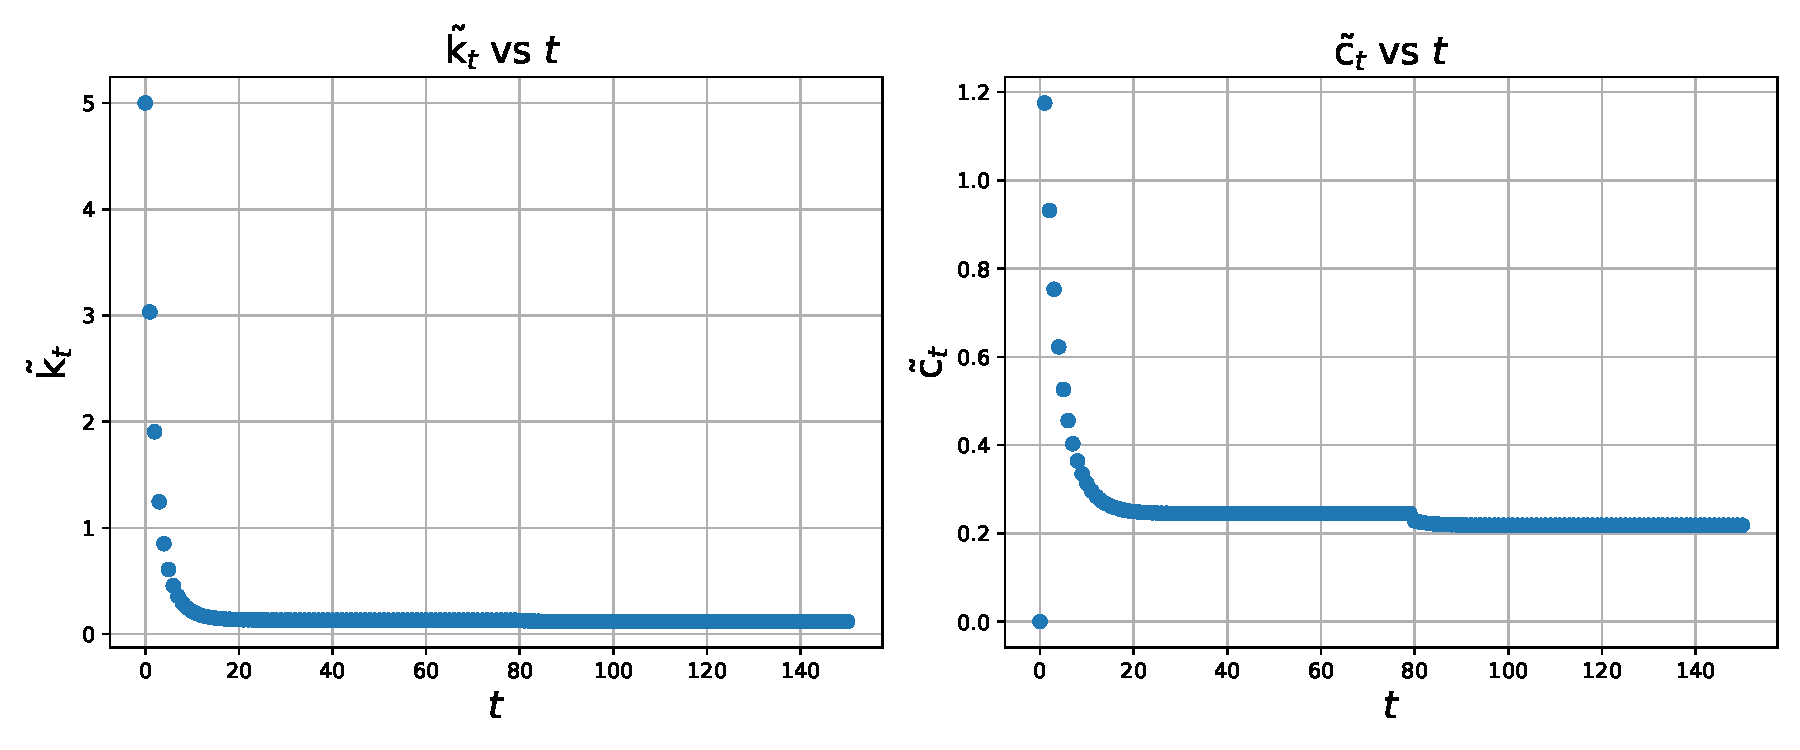
\includegraphics[width=1\textwidth]{4(g).pdf}
    \caption{Comparison of $\widetilde{k}_t$ (left) and $\widetilde{c}_t$ (right) under different 
    values of the tax rate $\tau$. Higher taxes reduce the resources available for private saving, 
    shifting the steady-state levels of both capital per effective worker and consumption per 
    effective worker.}
    \label{fig:4(g)}
\end{figure}

\end{document}

